\section{為什麼香港一天到晚都有示威遊行?}

因為正常代表民意的選舉和議會失效,就連傳媒也越來越不能反映社會多元意見。當人們無法在體制內表達不滿,不代表他們的訴求就會消失,也可能選擇在體制以外發聲。香港變成「示威之都」,側面反映民意反映制度本身的失效。

按香港警務處的統計,香港每年的公眾遊行和集會已有二零零八年的四千多宗增加至二零一八年的一萬一千多宗,或每日超過三十二宗。民間流行說的「三日一遊行,五日一示威」已是嚴重低估。有外國傳媒比較世界各地的數字,發現香港是世界上公眾抗議最頻密的城市,而且遠遠拋離第二位的墨西哥城。

\begin{figure}[htbp]
    \centering
    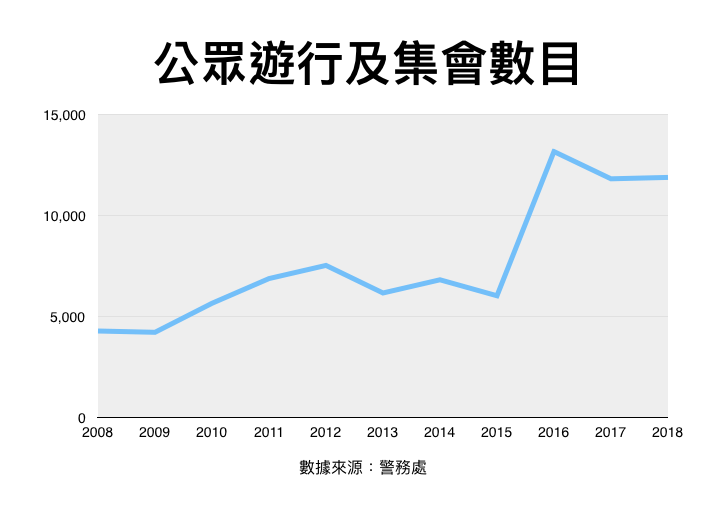
\includegraphics[width=0.7\textwidth]{c29/h-klesson1-046.png}
    \caption{遊行集會的數目越來越多} 
\end{figure}

遊行集會越來越多的原因有兩種可能。第一,參與者找不到更好的方法表達他們的訴求;第二,參與者起碼相信他們的表達有可能帶來一些改變(即使這些改變未必即時直接)。香港的情況符合上述兩點。議會在正常的情況下不能反映民意,不過在強大的壓力之下,如果有關鍵少數建制內的菁英願意裡應外合,或最少這些菁英發現利用當下的民意對他們有利,則仍有帶來改變的可能。二零零三年超過五十萬人上街的七一大遊行過後,本屬「執政聯盟」的自由黨毅然倒戈,使得政府不再有足夠票數通過國家安全立法,因而被迫撤回法案。自此之後,每年的七一遊行都會成為民間社會總動員的大日子,不同議題的組織都會趁當日出來表達訴求,和其他組織互相砥礪扶持,以及籌備處經費維持運作。

而由於香港的正規政治未能反映民意,有意見認為香港政府因此反而更受當下的民意所影響(見問題二十七)。這個民意並不是傳統意義下的「大多數人的意見」(反正政府不是由選舉產生),而是當下最能吸引大多數人注意力的聲音,可說是「響亮少數」。例如在清拆天星碼頭和皇后碼頭的爭議當中,雖然碼頭最終被拆,但政府及後更為強調歷史建築的「保育」,在公眾眼中也可視為「響亮少數」爭取所得的成果。這些經驗都說明了在「半民主」的政治體制下,集體行動與民意和正規政治之間的互動可帶來一定成果。

雖然遊行集會在香港已變得日漸普遍,但並不代表沒有困難。相反,無論在具體安排、發揮影響力,以及保持公眾關注這三方面,以遊行集會等抗議行動來表達訴求的困難可謂越來越多。

先說具體安排。按現行的《公安條例》, 50 人或以上的公眾集會或 30 人或以上的公眾遊行應事先通知警務處處長,得到「不反對通知書」後方可舉行。任何未經批准下進行公眾集會或公眾遊行即屬非法。而任何三人或以上集結在一起,意圖破壞社會安寧或者激使其他人破壞社會安寧,即犯非法集結。此等制度源於英治時期的高壓管治,當時社會上已有意見認為未能保障公眾的表達自由,認為管制過於嚴苛。特區成立後修訂《公安條例》時,法律學者陳文敏批評法例還原了殖民地的高壓管治,對維持社會安定沒有好處。

另一具體安排問題,是由誰來發起遊行集會。香港的遊行集會往往強調參與者的自發性,以免被親建制陣營的輿論批評參與者只是「被政客誤導」,事實上調查顯示參與者通常都是自發動員,不傾向由組織或團體動員。不過,實際上任何集體行動都需要一定程度的組織工作,例如佈置場地和與警察溝通,這些都要由各個非政府組織去做。香港法例保障結社自由,也有大量關注不同議題的非政府組織,他們都是組織集體行動的重要支柱。然而現時香港大多數的非政府組織都經營困難,而且難以成長。問題成因,也要回到香港政治制度的缺陷當中去解釋。在一個正常的民主社會當中,由於有政黨輪替,不同利益都要用各種方法保持對政府的影響力,民間的壓力和遊說團體有重要角色;但在香港的情況由於執政集團永遠執政,民間團體的影響力就難以得到證實,也就難以得到資源支持其工作,進以陷入欠缺資源和影響力的惡性循環。而由於在野的永遠在野,民間團體也和非建制陣營的政黨一樣面對碎片化的壓力。如是者,香港的民間社會便發展出很多微型團體,只能在重大議題時建立起反對政府的鬆散聯盟,卻難以發展成更強大持久的制衡力量。

互信不足帶來的問題在近年顯得更為明顯。舉個例,要辦一場大型活動難免會涉及一定開支,例如印刷場刊、場地租用、搭建舞台或租用擴音設備等。然而如果在會場籌款補貼這些開支,很容易就會被攻擊為「借社會運動發財」。即使組織者儘可能做到公開透明接受監督,但基於資源所限也難以滿足所有人的要求。因此,很多微型團體就被困在沒有資源就做不到良好內部管治,做不到良好內部管治就得不到更多資源的怪圈當中。

此外,香港於結社自由方面本來遠比中國大陸寬鬆,只要有三個人簽名提交一份兩頁紙的申請書就可註冊成為社團,又或直接去開一個商業公司登記,然後便可去銀行開立帳戶,沒有在中國大陸成立民辦非企業單位時要遇到的限制。不過,近年特區政府開始運用各種行政手段,為民間團體的運作製造困難。近年有多個民間組織如香港眾志和香港民族黨等因其政治立場而未能成功註冊,唯香港尚未就相關議題立法,政府拒絕註冊的法理基礎不明。後來政府更引用《社團條例》中「維護國家安全」的條文要求禁止香港民族黨運作,然而羅列出來的證據僅為其召集人的個人言論,沒有實際行動支持,被評為濫用相關條文和思想入罪。

至於遊行集會的影響力,近年也面對不少質疑。抗議行動特別是和平的抗議行動,出席人數往往是能構成多少公眾關注和壓力的重要指標,但是人數估算本身又往往會引起爭議,而參與者往種會質疑警方低估人數,而另一邊則會質疑主辦單位高估人數。警方對二零一四年和二零一六年就六四晚會的參與人數估計分別為99,500人和18,000人,唯兩次集會中人潮所佔的集會空間明顯沒有倍數之差,便引發了不少輿論質疑。為了就出席人數作客觀估算,有學者會用各種方法如會場人口密度來推算人數,香港大學民意研究計劃更多年來在七一遊行路線上架設攝錄鏡頭,然後人手點算經過人數,再推算出總出席人數。

其實任何有過萬人參加者的公眾集會,本質上已經應視為重大社會事件。不過有鑑於香港政治制度的缺陷,選舉結果本身不能準確反映民意,於是不少人會感到走上街頭表態然後讓各方點數得到他的出席,更能有效反映訴求。而傳媒也習慣以同一活動出席人數比去年的升跌,作為民意升溫或降溫的重要指標,進而引發出各方對點算人數的爭議和執著。就連政府或建制陣營於遊行同日舉辦大型嘉年華會,也會被視為要和遊行爭奪場地和出席人數。

另一個關於影響力的問題是當遊行集會越來越頻繁,會反過來變得難以保持公眾關注。學者李立峯和陳韜文以「社運社會」來形容集體行動在香港的常規化。他們指出社會運動作為爭取權益的模式已被越來越多的公民和團體採用,大眾對社會運動日漸變得習慣,或可說社會運動已被馴化,而這又反過來使社會運動失去了打破常規的能力,從而減少了對社會的影響力。

在一個很少人敢於發言的社會,如果有人走出來即使表達即使是最輕微的異議,例如到政府辦公的地方遞交意見書,已能突破社會常規吸引公眾關注。但當同樣的做法越來越多,關注也就難以持續,畢竟新聞關心的是有什麼「新」的東西。於是乎,異議者就要想出一些新的方法想吸引注意,例如在遞交意見時準備一些什麼道具,讓新聞畫面變得吸引一點。而最能突破社會常規的,當然就是一些相對激進的抗爭手法。在此,組織者往往要面對兩難:選擇公眾較為接受的形式,則其議題會被淹沒在其他形式相近的抗爭之中;選擇公眾未能接受的形式,雖然能達到吸引注意的效果,但其著眼點又可能會變成形式本身而非本來的議題。公眾可能會只顧譴責這些形式,而忽視為什麼這些人要出來表達意見。

與此同時,當行動不能帶來參與者預期的回報時,帶來的無力感也會打擊下一次參與的意欲。有意見認為零三年七一遊行的成功,拉高了公眾對參與遊行集會的期望。但當二零一四年的佔領運動未能帶來普選後,不同的運動參與者便互相指責對方不夠或過於激進,使得運動失敗。相關問題一直纏擾香港的公民社會,直到二零一九年的《逃犯條例》爭議,由「成效」之爭才開始被放下,回到「應做就去做」的初心。

最後,建制陣營也發展出一種應對遊行集會的方式:反動員操作。他們理解到上述各種舉辦遊行集會的困難和公眾的懷疑,便舉辦大量低質素的遊行集會來擴大這些質疑,使輿論對不論任何訴求的遊行集會都一律感到反感。例如他們在六四晚會或七一遊行期間也會安排反動員的集會,又或在立法會審議法案的時候發動群眾到場支持等等。這些活動的組織者的言行舉止往往比非建制陣營的更為激進,而參與者在傳媒面前又往往表現得連自己在參與什麼活動都不知道。不過,這些問題無損這些反動員活動,因為它們的目的並不是真的要表達支持或說服他人,而是要把表達意見這行為本身污名化。當一般人對政治議題和集體行動感到反感或最少厭煩,宏觀上就能達到維持現狀的目的,既得利益就可以持續。



伸延閱讀:

八十後自我研究青年(2013)《反抗就是罪名:政治檢控與盼望》,香港:香港基督徒學生運動。

李立峰、陳韜文(2013)〈初探香港「社運社會」— 分析香港社會集體抗爭行動的形態和發展〉,張少強,梁啟智,陳嘉銘編《香港.論述.傳媒》,香港:牛津大學出版社。

陳韜文、李立峰(2009)〈從民意激盪中重構香港政治文化:七一大遊行公共論述分析〉,馬傑偉、吳俊雄、呂大樂編《香港文化政治》,香港:香港大學出版社。

Ma N (2007) Civil Society in Self-Defense, \textit{Political Development in Hong Kong: State, Political Society}, and Civil Society. Hong Kong: Hong Kong University Press.